\documentclass[10pt,t, handout]{beamer} % handout
\usetheme{Heverlee}
\usepackage{animate}
\usepackage{tikz}
\usepackage{tikz-cd}
\usepackage{svg}
\usepackage{bm}

\usepackage[absolute, overlay]{textpos}

% notes
%\usepackage{pgfpages}
%\setbeameroption{show notes on second screen}
%\setbeamertemplate{note page}{%
%	\vskip 0pt
%	\lineskip 0pt
%	\normalsize
%	\insertnote
%}
\newcommand{\vk}{\vskip 5pt}
\newcommand{\press}{\textcolor{pblue}{PRESS}}
\usepackage{mathtools}

\newcommand{\R}{\mathbb{R}}

\setbeamertemplate{theorems}[numbered] 
\newtheorem{result}{Result}

%%% QUICK OPTIONS:
% (A) Math font without serifs, enable line below to make math serif:
    \usefonttheme[onlymath]{serif}

% (B) Re-define primary colour by adjusting the RGB values
%    \definecolor{pblue}{RGB}{206,125,66}

% (C) Title page graphic (optional) --- this is not for the background image, see \usebackgroundtemplate to change that ---
    %\titlegraphic{\includegraphics[height=2.7cm]{example_figure.pdf}}

% (D) Add logo to bottom right-corner (optional)
    \logo{\includegraphics[height=0.7cm]{media/icosahedron-src.pdf}\hspace{12pt}\vspace{-6pt}} 

% (E) Choose one (or none) of these lines to add footline bar on all frames
    %\setbeamertemplate{footline}[infoline]  % author, title, insitute
    %\setbeamertemplate{footline}[navigation] % dots swhowing progress
    %\setbeamertemplate{footline}[navsym] % navigation symbols

% (F) Widescreen 16:9 ratio
    %\usepackage[orientation=landscape,size=custom,width=16,height=9,scale=0.45,debug]{beamerposter} 

%%% TITLE PAGE INFO:

\title{Derived Commutativity in Data Science,\\ Category Theory, and Quantum Physics}
\subtitle{Theoretical and computational aspects}
\author[ammedmar]{Anibal M. Medina-Mardones}
\institute{Max Planck Institute for Mathematics}
\date{March 2021}

\begin{document}
{
% Change image, or delete this line to remove background image
\usebackgroundtemplate{ \parbox[b][\paperheight][b]{\paperwidth}{\centering\includegraphics[width=\paperwidth]{media/bg_alishan.jpg}}} 
 %   abudhabi      cherry      forest      river
 %   alishan       chobe       leuven      sanfancisco
 %   blueprint     columns     library     uyuni
 %   bokeh         flowers     newyork     winter

%\setbeamercolor{background canvas}{bg=lgray}  % make background light gray

% Title page
\begin{frame}[plain, noframenumbering]
	\note{Thank you, it's great to be here.}
    \titlepage
\end{frame}
}

% Table of contents slide
\begin{frame}{Outline}
	\note{This is the plan for today
	
	\vk

	I will start by describing how to associate certain topological invariants to data sets, I'll illustrate their use with a real world example, and introduce one of the computational tools available for their incorporation into machine learning.

	\vk
	
	In the next two section, I will explain how to effectively compute certain refinements of these topological invariants, and draw some connections to other fields: data science, sure, but also category theory and condensed matter physics.
	
	\vk
	
	I will then describe an abstract framework where these finer invariants are best understood, and present some computational and theoretical advances in this context.
	
	\vk
	
	Finally, I will return to applications, and present a novel use of topological methods in information theory.
	}

	\vskip 2mm
	\hfill{\large \parbox{.95\textwidth}{\tableofcontents[hideothersubsections]}}
\end{frame}

\section{From data to topology}
\note{Let's start here. And if you would like a handout version of the slides, I am placed the link the chat.}

\begin{frame}{Point clouds}
	\note{\small
		We can think of a point cloud of data, as obtained by sampling from a probability distribution function on $\R^n$.
		\vk
		These tend to concentrate around lower dimensional subspaces, like in this idealized picture.
		\vk
		We would like to have ways to approximate and study this underlying space. \press
		\vk		
		Let me describe a method we can use to approximate this.
		Given a scale parameter $r$, we construct a triangulation as follows.		
		We join, with an edge, pairs of points in the cloud if their distance is less that $r$, the fixed parameter.
		If 3 points have pairwise distances less than $r$, then we place a triangle between them, and for 4 points, we include tethrahedra and so forth. 
		\press
		
		Here we see 4 examples of triangulations constructed over the same dataset with increasing values of the parameter.
		\vk
		But, instead of picking a scale, corresponding to a specific value of the parameter, we can consider the entire family of approximations, noticing that there is structure in this family. \press
		\vk
		If $r$ is less than $r^\prime$, then the approximation at scale $r$ is part of that at $r^\prime$.
		\vk
		We will exploit this coherence after we overview a key topological invariant we can construct for any triangulated space.
		I am refering to Homology. 
	}
	A data set can often be thought of as a point cloud in $\R^n$.
	
	\vskip 8pt
	
	Underlying probability distribution concentrated in a subspace.
	
	\vskip -5pt
	
	\begin{center}
		\includegraphics[scale=.3]{media/torus}
	\end{center}
	
	\pause 
	
	How to approximate and study the underlying shape?
	
	\pause
	\vskip 5pt
	
	\begin{center}
		\includegraphics[scale=.4]{media/filtration}
	\end{center}
	
	\pause
	\vskip-10pt
	\textcolor{pblue}{Multi-scale approximation}
\end{frame}

\begin{frame}[c]{Homology}
	
	\note{\footnotesize Given simplicial complex, for example, a fixed scale approximation to a data set, or just some some graph.
	We are after invariants of it that are preserved under deformations and, therefore, are robust to noise in the data.
	Homology is one such invariant, which generalizes the well known Euler characteristic of a graph.
	To define it, let us first encode the incidence relations of our simplicial complex in terms of binary matrices. \press
	
	Let's take this example. By convention, the matrix associated to vertices is 0. For edges, it agrees with the well known incidence matrix of the underlying graph. For 2-dimensional simplices it tells us what edges are part of its boundary. For higher dimensional simplices we have the analogous situation encoding what codimension 1-simplices are part of their boundary. This explains the name of these matrices: the boundary matrices of a simplicial complex. \press
	
	We now define, for every non-negative integer $n$, the vector space $H_n$, known as the the $n$-th homology of $X$, as the quotient of the kernel of the $n$-boundary matrix and the image of the $(n+1)$-th one. We are particularly interested in the rank of this vector space, which we call the $n$-th betti number.
	These betti numbers are constructed using linear algebra, and they are highly computable.
	The 0 betti number is nothing but the number of connected componets of $X$, whereas the 1 betti number is the number of non-contractible independent cycles in $X$. The higher betti numbers count higher-dimensional cavities. These are powerful and computable signatures of $X$.
	For example, any triangulation of sphere-like shape will have betti number 1 equal to 0, whereas for any torus-like shape it will be 2. This implies the original shapes cannot be continuously deformed one into the other. \press
	
	The last important point I want to make is that if we have an inclusion of simplicial complexes, then we get a linear map between their homologies. We will use this to parameterize the homology costruction so to treat all scales simultaneously in the case of a point cloud.
	
	Let us return to that family of simplicial complexes approximating the shape of data.
}
	
	\vskip -15pt
	
	Given a simplicial complex $X$
	\begin{center}
		\includegraphics[scale=.05]{media/simplicial_complex}
		\qquad\qquad
		\pause
		\includegraphics[scale=.8]{media/simplex}
	\end{center}
	
	Incidence relations as a matrices
	
	\begin{equation*}
	\partial_0 =
	\begin{pmatrix}
	0 & 0 & 0 
	\end{pmatrix}
	\qquad
	\partial_1 =
	\begin{pmatrix}
	1 & 1 & 0 \\
	1 & 0 & 1 \\
	0 & 1 & 1 
	\end{pmatrix}
	\qquad
	\partial_2 =
	\begin{pmatrix}
	1 \\
	1 \\
	1 
	\end{pmatrix}
	\end{equation*}
	
	\vskip 5pt
	\pause
	
	\textcolor{pblue}{Definition:} $\displaystyle{H_n(X; \mathbb F_2) = \frac{\ker \partial_n}{\mathrm{im}\, \partial_{n+1}}}$ \quad Its rank denoted $\beta_n$.
	
	\vskip 15pt
	\pause
	
	\textcolor{pblue}{Naturallity:}	
	If $X \subseteq X^\prime$ then $H_n(X; \mathbb F_2) \to H_n(X^\prime; \mathbb F_2)$
\end{frame}

\begin{frame}{Persistence homology}
	
	\note{Persistence homology arises by quantifying the way the ranks of the induce linear maps fit together. By taking $s = t$ we just get back the betti numbers of the simplicial complex at that scale, but there is much more information available. \press
	
	We mentioned that the 0-betti number counts the number of connected components.
	So, for parameter $r = 0$ we have as many components as points in the cloud. But, as we increase the value of $r$ these points start connecting and the number of components decreases until, eventually, all points are connected.
	The invariant associated to persistence 0-homology encodes precisely how long connected components last before merging.
	This invariant is known in data science as the hierarchical clustering diagram of the point cloud. \press 
	
	We can think of the invariants associated to persistence $n$-homology, known as the $n$-th persistence diagram, as econding the life span of $n$-dimensional cavities in the data. \press
	
	To recap then, we have a the following pipeline:
	
	Given a point cloud, we produce a multi-scale coherent family of approximations to some underlying space of the data. Then, we associate linear algebra computations to it,	which produces multiscale topological invariants generalizing a well know construction in machine learning.
	\vk
	I will now overview a remarkable and in some ways paradigmatical application of this pipeline to material science.
	}

	\vskip -5pt
	
	Quantifies the ranks of the linear maps $H_n(X_s) \to H_n(X_t)$ for $s \leq t$.
	
	\vk\vk
	\pause
	
	\textcolor{pblue}{Machine Learning Intuition:}
	
	\vk
	
	\textbf{Q}: What does keeping track of how $\beta_0$ changes with $r \in \R_{\geq 0}$ tells us?
	
	\pause
	\vk
	
	\textbf{A:} Hierarchical clustering.
	
	\begin{center}
		\includegraphics[scale=.2]{media/dendogram}
	\end{center}

	\pause
	\vskip -10pt
	
	\textcolor{pblue}{Pipeline:}
	\begin{center}
		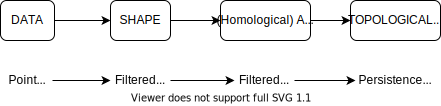
\includegraphics[scale=.8]{media/diagram.pdf}
	\end{center}
\end{frame}

\begin{frame}{Example: nanoporous materials}
	
	\note{
	It was done by these researchers. including, Kathryn Hess, a leading figure in the community who runs the Topology and Neuroscience lab at EPFL. She will come back to the story later. \press
	\vk
	This researchers focused on nanoporous materials. These consist of an organic or inorganic framework supporting a regular porous structure. Tipically, the size of the pores is 100 nanometers or smaller.
	There are a lot of such materials, and many more are being made inrapid succesion.
	Naturally, the chemical composition is very important, but also the geometric structure of the pores, which as been probed with tools from christallography and other fields. \press
	\vk
	But what about Topology?
	}

	\textcolor{pblue}{Work by:} Lee, Bartel, Dlotko, Moosavi, \underline{Hess}, Smit
	
	\begin{center}
		\includegraphics[scale=.085]{media/hess}
	\end{center}
	
	\pause
	
	\begin{itemize}
		\item Large database of nanoporous materials.
	
		\vk
		
		\item Geometry of pore structure affects their properties (e.g. methane storage), even when the chemistry is unchanged.
		
		\vk
		
		\item Conventional descriptors look at crystallographic structure, sizes of embedded spheres, and others.
	\end{itemize}
	
	\vk
	\pause
	
	\textcolor{pblue}{What can persistence homology say?}	
\end{frame}

\begin{frame}{Example: nanoporous materials}
	
	\note{There is a catalogue of over 3 million nanoporous structures. One would like to compare the geometries of these, but direct inspection on a data of this size is out of the question.
	\vk
	The authors constructed persistence diagrams using dimensions 0, 1 and 2 for each of these nanoporous structure. They used the methods we discussed starting with a point cloud of equidistantly distributed points in the cavities of a fundamental domain.
	\vk
	Since the set of persistence diagrams can be made into a metric space, they were able to quantify the distance of nanoporous geometries, using the distance of their associated persistence diagrams. \press
	\vk
	The authors were able to identify in this way materials with very similar nanoporous structures missed by other methods. Here are some examples. In each row there are distinct nanoporous materials that were identified to be have very similar geometries.
	\vk
	As an application of the gain insight, they showed wrong a belief about the relationship between methane storage capabilities and the heat of absortion of a material. 
	}
	\textcolor{pblue}{Comparing geometries:} \\
	Over 3M structures.
	
	\begin{textblock*}{4cm}(5.4cm,1.5cm)
		\includegraphics[scale=.28]{media/real_material}
	\end{textblock*}
	
	\pause
	\vspace*{2cm}
	
	\textcolor{pblue}{Vectorisation method:} \\
	Persistence diagrams \\
	are a metric space.
	
	\vspace*{-1cm}
	\hspace*{3.8cm}\includegraphics[scale=.6]{media/nanoporous}
\end{frame}

\begin{frame}{Machine Learning and Topology}
	
	\note{We have seen how persistence homology provides interesting new features of data sets. But, up to recently, most software available for their computation was written by and for TDA experts.
	
	With two goals in mind: one, to improve the speed of persistence homology computations AND, two, to integrate it into the traditional pipelines of machine learning. A collaboration between the Topology and Neuroscience Lab at EPFL, High performance experts from the REDs institute, and the Swiss machine learning company L2F, we developed giotto-tda. \press
	\vk
	A Python package for TDA built on top of high performance C++ code, that closely follows the operational structure of scikit-learn, and integrates effortlessly into machine learning pipelines.
	\vk
	This open source project also makes available several learning resources from its documentation page. The place I would recommend visiting to check if these tools can be used in your data science project.
	}
	
	Is topological data analysis \textcolor{pblue}{only} for the experts?
	\pause
	\textcolor{pblue}{Not anymore.}
	
	\vskip 10pt
	
	\includegraphics[scale=.33]{media/giotto}	
\end{frame}

\section{Finer invariants}
\note{How can we go beyond homology? For the next 15 minutes I will assume some familiarity with topology, but will return to an application I led during the last 5 minutes of this talk.}

\begin{frame}{Finer topological invariants}
	\note{
	Let us motivate the need for finer invariants by considering two spaces: the Torus and the Klein bottle. We obtain them by gluing together the edges of these squares following the patterns defined by the displayed arrows. Torus on the left, Klein bottle on the right.}	
	
	\newcommand*{\xMin}{0}%
	\newcommand*{\xMax}{4}%
	\newcommand*{\yMin}{0}%
	\newcommand*{\yMax}{4}%
	\begin{center}
	\begin{tikzpicture}[scale=.6]
	\draw[-{Latex[length=2mm]}] (-.5,\yMin)--(-.5,\yMax);
	\draw[-{Latex[length=2mm]}] (-.5,\yMin)--(-.5,\yMax-.5);
	\draw[-{Latex[length=2mm]}] (4.5,\yMin)--(4.5,\yMax);
	\draw[-{Latex[length=2mm]}] (4.5,\yMin)--(4.5,\yMax-.5);
	
	\draw[-{Latex[length=2mm]}] (\xMin, -.5)--(\xMax, -.5);
	\draw[-{Latex[length=2mm]}] (\xMin, 4.5)--(\xMax, 4.5);
	
	\draw (0,0)--(0,4)--(4,4)--(4,0)--(0,0);
	
	\node at (2,-1.2){$T$};
	\end{tikzpicture}
	\hspace*{2cm}
	\begin{tikzpicture}[scale=.6]
	\draw[-{Latex[length=2mm]}] (-.5,\yMin)--(-.5,\yMax);
	\draw[-{Latex[length=2mm]}] (-.5,\yMin)--(-.5,\yMax-.5);
	\draw[-{Latex[length=2mm]}] (4.5,\yMax)--(4.5,\yMin);
	\draw[-{Latex[length=2mm]}] (4.5,\yMax)--(4.5,\yMin+.5);
	
	\draw[-{Latex[length=2mm]}] (\xMin, -.5)--(\xMax, -.5);
	\draw[-{Latex[length=2mm]}] (\xMin, 4.5)--(\xMax, 4.5);
	
	\draw (0,0)--(0,4)--(4,4)--(4,0)--(0,0);
	
	\node at (2,-1.2){$K$};
	\end{tikzpicture}
	\end{center}
\end{frame}

\begin{frame}{Finer topological invariants}
	
	\note{
	With mod 2 coefficients the betti numbers cannot distinguish them, although they are topologically inequivalent as the following geometric argument shows:
	The self intersection number of a basis cycle in the torus is always even, we can slide the cycle off of itself. But, for the Klein bottle, this is not true, as this picture illustrates.
	
	We would like to algebraically capture this topological twisting. We can do so by endowing cohomology with further algebraic structures: \press 
	
	either an algebra structure or a module structure over the Steenrod algebra.
	
	I will define these in the next slides, emphasising how they are both induced from a structure at the cochain level, the matrix level.
	\vk
	Before going there though, a quick comment for the experts, in case you are wondering about coefficients here, notice that we can replace the torus and the Klein bottle by $\mathbb CP^2$ and the wedge of a 4 and a 2 sphere to make the same point over the integers. Yet, mod 2 coefficients are preferable in many applications since they can be stored with just one bit.
	\vk
	Let us return now to the definition of this extra algebraic structure on cohomology, the linear dual of homology.
}
	
	\newcommand*{\xMin}{0}%
	\newcommand*{\xMax}{4}%
	\newcommand*{\yMin}{0}%
	\newcommand*{\yMax}{4}%
	
	\begin{center}
	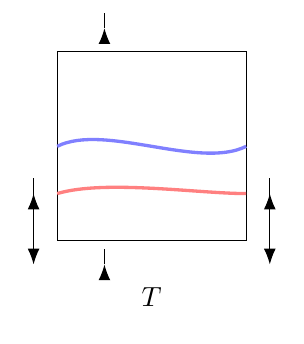
\begin{tikzpicture}[scale=.6]
	\draw[-{Latex[length=2mm]}] (-.5,\yMin)--(-.5,\yMax);
	\draw[-{Latex[length=2mm]}] (-.5,\yMin)--(-.5,\yMax-.5);
	\draw[-{Latex[length=2mm]}] (4.5,\yMin)--(4.5,\yMax);
	\draw[-{Latex[length=2mm]}] (4.5,\yMin)--(4.5,\yMax-.5);
	
	\draw[-{Latex[length=2mm]}] (\xMin, -.5)--(\xMax, -.5);
	\draw[-{Latex[length=2mm]}] (\xMin, 4.5)--(\xMax, 4.5);
	
	\draw (0,0)--(0,4)--(4,4)--(4,0)--(0,0);
	
	\draw[color=blue!50, very thick] (0,2) .. controls (1,2.5) and (3,1.5) .. (4,2);
	\draw[color=red!50, very thick] (0,1) .. controls (1,1.3) and (3,1) .. (4,1);
	
	\node at (2,-1.2){$T$};
	\end{tikzpicture}
	\hspace*{2cm}
	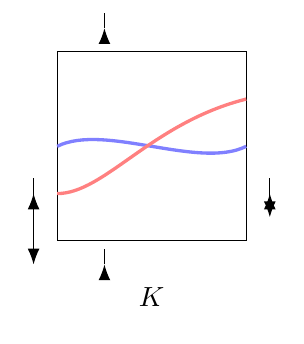
\begin{tikzpicture}[scale=.6]
	\draw[-{Latex[length=2mm]}] (-.5,\yMin)--(-.5,\yMax);
	\draw[-{Latex[length=2mm]}] (-.5,\yMin)--(-.5,\yMax-.5);
	\draw[-{Latex[length=2mm]}] (4.5,\yMax)--(4.5,\yMin);
	\draw[-{Latex[length=2mm]}] (4.5,\yMax)--(4.5,\yMin+.5);
	
	\draw[-{Latex[length=2mm]}] (\xMin, -.5)--(\xMax, -.5);
	\draw[-{Latex[length=2mm]}] (\xMin, 4.5)--(\xMax, 4.5);
	
	\draw (0,0)--(0,4)--(4,4)--(4,0)--(0,0);
	
	\draw[color=blue!50, very thick] (0,2) .. controls (1,2.5) and (3,1.5) .. (4,2);
	\draw[color=red!50, very thick] (0,1) .. controls (1,1) and (2,2.5) .. (4,3);
	
	\node at (2,-1.2){$K$};
	\end{tikzpicture}
	\end{center}
	
	Although $H^\bullet(T, \mathbb F_2) \cong H^\bullet(K, \mathbb F_2)$ as graded vector spaces $T \not\cong K$.
	
	\vskip 5pt
	\pause
	There is more algebraic structure that distinguishes them
	\begin{align*}
	\smallsmile & \colon H^\bullet \otimes H^\bullet \to H^\bullet && \text{(commutative ring structure)},\\
	Sq^k & \colon H^\bullet \to H^\bullet && \text{(module over Steenrod algebra)}.
	\end{align*}
\end{frame}

\begin{frame}[fragile]{Alexander-Whitney \& Steenrod}
	
	\note{The cup product in cohomology was defined in the 30's by Alexander, Kolmogorov, \v{C}ech and Whitney, dualizing a chain approximation to the diagonal map.
	
	Although the resulting cup product in cohomology is graded commutative, the cup-0 product of cochains it's not. We can see that by just transposing the factors in this tensor product. We get a different formula.
	
	Steenrod, in the late 40's, introduced a correction to the lack of commutativity of cup-0 in the form of another explicit product, \press
	
	cup-1. It satisfies that the coboundary of cup1 is equal to the difference between cup-0 and its transpose. This right hand side would be 0 if cup-0 were commutative, which is not, but what we have is that cup0 is commutative up to an explicit coboundary given by cup-1.
	\vk
	We notice some symmetry here, because, after transposing this identity, that is permuting alpha and beta, we see that the coboundary of the transpose of cup1 is also equal to the right hand side of this identity. Cup-1 and its transpose, both enforcing the derived commutativity of cup-0, are in general not equal to each other.}

	\vskip -5pt
	The cup product
	\begin{equation*}
	\smallsmile \colon H^\bullet \otimes H^\bullet \to H^\bullet,
	\end{equation*}
	\vskip -9pt
	defined via
	\vskip -9pt
	\begin{equation*}
	\smallsmile_0 \colon C^\bullet \otimes C^\bullet \to C^\bullet,
	\end{equation*}
	dual to 
	\begin{equation*}
	\begin{tikzcd}[
	,row sep = 0ex
	,/tikz/column 1/.append style={anchor=base east}
	,/tikz/column 2/.append style={anchor=base west}
	]
	C_\bullet \arrow[r, "\Delta"] & C_\bullet \otimes C_\bullet \\
	{[0, \dots, n]} \arrow[r, |->] & \sum_{i=0}^{n} {[0, \dots, i] \otimes [i, \dots, n]}.
	\end{tikzcd}
	\end{equation*}
	
	\vskip 15pt
	\pause
	
	\textcolor{pblue}{Steenrod's cup-$1$:} \quad
	$\delta(\alpha \smallsmile_1 \beta) = \alpha \smallsmile_0 \beta\, -\, \beta \smallsmile_0 \alpha$ 
\end{frame}

\begin{frame}[fragile, noframenumbering]{Alexander-Whitney \& Steenrod}
	
	\note{So Steenrod constructed an explicit cup-2 product to correct for this, making cup-1 commutative up to an explicit coboundary.
	}
	
	\vskip -5pt
	The cup product
	\begin{equation*}
	\smallsmile \colon H^\bullet \otimes H^\bullet \to H^\bullet,
	\end{equation*}
	\vskip -9pt
	defined via
	\vskip -9pt
	\begin{equation*}
	\smallsmile_0 \colon C^\bullet \otimes C^\bullet \to C^\bullet,
	\end{equation*}
	dual to 
	\begin{equation*}
	\begin{tikzcd}[
	,row sep = 0ex
	,/tikz/column 1/.append style={anchor=base east}
	,/tikz/column 2/.append style={anchor=base west}
	]
	C_\bullet \arrow[r, "\Delta"] & C_\bullet \otimes C_\bullet \\
	{[0, \dots, n]} \arrow[r, |->] & \sum_{i=0}^{n} {[0, \dots, i] \otimes [i, \dots, n]}.
	\end{tikzcd}
	\end{equation*}
	
	\vskip 15pt
	
	\textcolor{pblue}{Steenrod's cup-$2$:} \quad
	$\delta(\alpha \smallsmile_2 \beta) = \alpha \smallsmile_1 \beta\, -\, \beta \smallsmile_1 \alpha$
\end{frame}

\begin{frame}[fragile, noframenumbering]{Alexander-Whitney \& Steenrod}
	
	\note{This process continues resulting in the cup-$i$ products of Steenrod: a coherent collection of explicit products whose coboundaries correct the lack of commutativity of the previous correction.
		
	Now, this structure on cochains defines at the cohomology level not just the cup product, but also the celebrated Steenrod squares. \press
	
	The importance in stable homotopy theory of this operations is hard to overstate.
	\vk
	If we want to compute them in specific cases though, we need to use the cup-$i$ products.
	
	I will argue that these are also quite important.
	}
	
	\vskip -5pt
	The cup product
	\begin{equation*}
	\smallsmile \colon H^\bullet \otimes H^\bullet \to H^\bullet,
	\end{equation*}
	\vskip -9pt
	defined via
	\vskip -9pt
	\begin{equation*}
	\smallsmile_0 \colon C^\bullet \otimes C^\bullet \to C^\bullet,
	\end{equation*}
	dual to 
	\begin{equation*}
	\begin{tikzcd}[
	,row sep = 0ex
	,/tikz/column 1/.append style={anchor=base east}
	,/tikz/column 2/.append style={anchor=base west}
	]
	C_\bullet \arrow[r, "\Delta"] & C_\bullet \otimes C_\bullet \\
	{[0, \dots, n]} \arrow[r, |->] & \sum_{i=0}^{n} {[0, \dots, i] \otimes [i, \dots, n]}.
	\end{tikzcd}
	\end{equation*}
	
	\vskip 15pt
	
	\textcolor{pblue}{Steenrod's cup-$i$:} \quad	
	$\delta(\alpha \smallsmile_i \beta) = \alpha \smallsmile_{i-1} \beta\, -\, \beta \smallsmile_{i-1} \alpha$
	
	\vskip 15pt
	\pause
	
	\textcolor{pblue}{Steenrod's squares:}
	
	\vskip -15pt
	\begin{equation*}
	\begin{tikzcd}[
	,row sep = 0ex
	,/tikz/column 1/.append style={anchor=base east}
	,/tikz/column 2/.append style={anchor=base west}
	]
	H^\bullet \arrow[r, "Sq^k"] & H^\bullet \\
	{[\alpha]} \arrow[r, |->] & {\left[\alpha \smallsmile_{k-|\alpha|} \alpha\right]}.
	\end{tikzcd}
	\end{equation*}
\end{frame}

\begin{frame}[c]{Cup-$i$ products}
	
	\note{\footnotesize
	Although, in principle there are many choices for the cup-$i$ products defining the same squares, every time the these have been constructed, the resulting formulas recover Steenrod's original definition of the cup-$i$ products. There seem to be interesting reasons for this. \press
	
	The first result I want to present, tells us that a few natural constrains completely determine the cup-$i$ products.
	
	I like to think of this result in analogy with harmonic representatives in de Rham theory of Riemannian manifolds. Many differential forms represent the same cohomology class, but there is a preferred one, the one picked by the geometry. \press
	\vk
	In proving this result, a new description of the cup-$i$ products was needed.
	These new formulas lead to much more efficient computations over simplicial complexes, and are the basis for the use of Steenrod squares in persistence homology.
	
	Using a pretty sub-optimal implementation of my algorithms we have already seen non-trivial persistence Steenrod squares in real-world data. The full potential of this technique will soon be seen after we finish a high performance implementation of it with rest of giotto-tda's team.
	\vk
	
	The next result is a bit further out there, but, given the strenght of this department in higher category theory, I wanted to mention a theorem that connects the axiomatized cup-$i$ products with a fundamental construction in that field. \press
	
	I constructed a functor from certain algebras with cup-$i$ products to $\omega$-categories, and showed that this functor sends the cochains on a standard simplex equipped with Steenrod's cup-$i$ products, to the free $\omega$-category generated by that simplex, the so called Street oriental. These orientals define the nerve of $\omega$-categories, which, via complicial sets, provides a definition of infinity categories.\\}

	\vskip -10pt
	\pause
	\begin{result}[Medina-Mardones]
		Just like the $Sq^k$ can be axiomatized, the $\smallsmile_i$ can be as well, and\\ all known constructions satisfy these axioms.
	\end{result}

	\pause
	\vskip 10pt
	
	\begin{result}[M-M]
		New description of the $\smallsmile_i$-products leading to \\
		incorporation of $Sq^k$ into persistence homology, and \\
		high performance version under development (w/ giotto-tda's team).
	\end{result}
	
	\pause
	\vskip 10pt
	
	\begin{result}[M-M]
		The $\smallsmile_i$-products determine another fundamental construction: the nerve of $\omega$-categories.
	\end{result}
\end{frame}

\section{Even finer invariants}
\note{Let's discuss some even finer invariants of the cohomology of spaces}

\begin{frame}{Secondary operations}
	\note{Steenrod squares are defined by the cup-$i$ products which arise from lifting to the cochain level the commutativity relation of the cup product in cohomology. Recall, that the coboundary of cup-1 is the difference between cup-0 and its transpose.
	
	We are motivated then to look for other cohomological relations to lift.
	
	We look at Steenrod squares themselves, sometimes referred to as primary cohomology operations. They satisfy relations and the invariants that appear by lifting and solving these relations are known as secondary operations. \press
	
	There are two main relations that Steenrod squares satisfy: The Cartan and Adem relations. The first tells us how the squares interact with the cup product and the second tells us about their behaviour under interation. \press
	
	Can we lift these relations the cochain level?
	
	Yes, the cup-$i$ products can be used to define both, the squares and the cup product in cohomology, so we use them to express these relations in the form: cup-$i$ version of the left hand side minus cup-$i$ version of the right hand side equal to a coboundary \press
	
	So we wonder if we can solve these equation, effectively constructing such coboundaries, and unlocking secondary cohomology operations
}
	
	The $Sq^k$ are obtained from lifting the relation
	\begin{equation*}
	[\alpha] \smallsmile [\beta] = [\beta] \smallsmile [\alpha].
	\end{equation*}
	
	\pause
	
	What are \textcolor{pblue}{their} relations?	
	\begin{align*}
	& Sq^k(\alpha \smallsmile \beta) = \sum_{i+j=k} Sq^i(\alpha) \smallsmile Sq^j(\beta), &&
	\text{(Cartan relation)} \\	
	& Sq^i Sq^j(\alpha) = \sum_{k=0}^{\lfloor i/2 \rfloor} {j-k-1 \choose i-2k} Sq^{i+j-k} Sq^k(\alpha) &&
	\text{(Adem relation)}
	\end{align*}
	
	\pause
	\vskip 5pt
	\textcolor{pblue}{Can we lift these relations?} \pause
	Yes: 
	\begin{equation*}
	C_k = \delta X, \qquad A_{i,j} = \delta Y,
	\end{equation*}
	\textcolor{pblue}{Can we solve them?}
\end{frame}

\begin{frame}[c]{Relations}
	
	\note{Another source of motivation for this question, and actually the original motivation for me, came from physicits studing exotic states of matter and other aspects of lattice field theory. \press
	
	Anton Kapustin from Caltech asked for a cochain level proof of the Cartan relation to have acces to these Cartan coboundaries, and they, together with Ryan Torngren now at Harvard, use some of my formulas in their work.
	
	\vk
	
	The question about Adem relations needed more ideas \press\
	and we tackle that project in collaboration with Greg Brumfiel from Stanford and John Morgan from Columbia.
}
	
	\pause 
	
	\begin{result}[M-M]
		Effective construction of Cartan coboundaries.
	\end{result}

	Work motivated by physicist A. Kapustin (Caltech) and R. Thorngren (Harvard). They used my formulas in lattice field theory.
	
	\begin{center}
		\includegraphics[scale=.13]{media/kapustin}
		\hspace*{1cm}
		\includegraphics[scale=.21]{media/thorngren}
	\end{center}
	
	\pause
%	\vskip 20pt
	
	\begin{result}
		Effective construction of Adem coboundaries.
	\end{result}

	The above is joint with G. Brumfiel (Stanford) and J. Morgan (Columbia).
	
	\begin{center}
		\includegraphics[scale=.21]{media/brumfiel}
		\hspace*{1cm}
		\includegraphics[scale=.09]{media/morgan}
	\end{center}
\end{frame}

\begin{frame}{Odd primes}
	
	\note{So far we have talked about Steenrod operations at the even prime. What about Steenrod operations for cohomology with general mod $p$ coefficients?
	
	These operations were defined indirectly by Steenrod, using group cohomology, and not through an effective construction analogue to the cup-$i$ products.
	
	For most application is abstract homotopy theory, we do not need effective constructions, but the applications of these ideas in the novel contexts I have outlined require them. \press
	
	So, with Ralph Kaufmann from Purdue, we generalized the cup-$i$ products to multivariate products responsible for Steenrod operations at any prime.
	
	\vk
	\vk
	
	Looking at all the results I have mentioned in this ``even finer invariants section", it is natural to wonder, what made these advances possible \textit{now}. Why weren't they solved during Steenrod's time. \press
	
	I have alluded already to the fact that one can do a whole lot with cohomology operations staying at the cohomology level. So there wasn't a big motivation to work at the cochain level. But, on top of the new applications, and the associated motivation that comes with them, the technical advances needed were developed as part of the theory of operads. }
	
	So far we have focused on $\mathbb{F}_2$ coefficients.
	
	\vskip 5pt
	
	What about \textcolor{pblue}{odd} primes?
	
	\pause
	\vskip 5pt
	
	\begin{result}
		Effective constructions of generalizations of the $\smallsmile_i$-products to odd primes.
	\end{result}
	Joint with R. Kaufmann (Purdue).
	
	\begin{center}
		\includegraphics[scale=.1]{media/kaufmann}
	\end{center}
	
	\pause
	\vskip 9pt
	
	\textcolor{pblue}{What made these advances possible?}
	
\end{frame}

\section{The operadic viewpoint}
\note{So let me say just a few words about this.}

\begin{frame}{Operads}
	
	\note{\footnotesize
	A useful analogy for operads is based on group theory. If we only care about group representations, and we did not know about abstract groups, we might stay in the context of vector spaces with a chosen set of automorphisms. But we know that this structure can be abstracted, and in many cases should be. \press
	
	Similarly, we can think of operads as the abstracted theory of algebras; commutative, Lie, or associative among others. \press
	
	If we mix this with notions from homotopy theory. Now a days we think of the derived notion of a commutative algebra, as an algebra over an $E_\infty$-operad. With the definition of an $E_\infty$-operad given only up-to-homotopy, like the definition of the classifying space of principal $G$-bundles, for example.

	So, we can interpret some of the advances I outlined during the previous part of the talk, using the fact that cochains of spaces are examples of $E_\infty$-algebras over certain effective models of the $E_\infty$-operad. \press
	
	To make the study of these models and their algebras easier, \press
	
	I wrote a specialized computer algebra system where some of the effective constructions I described are implemented at the operad level, applying in particular to cochains of spaces.
	
	This is an open source project with thorough documentation and an easy installation step.
	
	\vk
	A final result I want to share, a bit technical I am afraid, is the construction of a new model of the $E_\infty$-operad. \press
	
	No finitely presented $E_\infty$-operad can exist, but passing to the more general context of props allowed me to finitely present a prop whose associated operad is a model of $E_\infty$. Furtheremore, it is cofibrant in the model category of operad, and it has an action on cochains of spaces generalizing the previously known $E_\infty$-algebra structures on them.\par}
	
	\vskip -5 pt
	\pause
	
	\textcolor{pblue}{Analogy}:	abstract groups are to group representations as	\\
	Operads are to algebras (commutative, or Lie, or associative, or $\dots$)	
	
	\vskip 5 pt
	\pause
	
	\textcolor{pblue}{Derived version} of commutative algebra: algebra over an $E_\infty$-operad.
	
	\vskip 5 pt
	\pause
	
	There are effective models due to McClure-Smith and Berger-Fresse.
	
	\pause
	
	\begin{result}[M-M]
		A computer algebra system on Python for the study of these operads and their algebras. (Right place to implement some of the earlier results).
	\end{result}
	
	\vskip 5 pt
	\pause
	
	More theoretically,
	
	\begin{result}[M-M]
		Although no finitely presented $E_\infty$-operad can exist, I constructed a finitely presented prop $\mathcal M$ whose associated operad is $E_\infty$. Furthermore, \\
		this operad is cofibrant and compatible with previous models.		
	\end{result}
\end{frame}

\section{Back to data}
\note{I would like to finish by tell you about a project I lead, using topological methods in the study of complex systems and information theory}

\begin{frame}{Graph Laplacian}
	
	\note{The graph Laplacian has become a primary tool for the study of networks. 
	\vk
	It is typically defined using the incidence matrix of a graph and the valence matrix of its nodes, but we can equivalently define it using the boundary matrix that gave us 1-homology. \press
	
	Here is the definition and an example illustrating it.
	\vk
	Naturally, we can set $W$ to be the identity if we are interested in unweighted networks. \press
	
	The spectrum of this matrix is an important feature of the network. \press
	
	Additionally, we can consider the eigenvectors of the graph Laplacian. This preferred basis is often used for signal analysis on graphs. \press 
	
	Where \textit{signal} in this context means a real-valued function from the set of vertices of the graph. \press

	What if we are interested in signals defined not just on vertices but on sets of such vertices? But even earlier, are there any interesting signals defined on subsets of vertices?
	}
	
	A powerful tool to study weighted networks. 
	
	\vskip 5pt
	\pause
	
	\begin{center}
		\includegraphics[scale=.5]{media/graph}
	\end{center}
	
	\vskip -5pt
	
	\begin{equation*}
	\resizebox{8.5cm}{!}{
		$\partial_1 =
		\begin{pmatrix*}[r]
		-1 & -1 &  0 \\
		 1 &  0 & -1 \\
		 0 &  1 &  1
		\end{pmatrix*}
		\qquad
		W =
		\begin{pmatrix*}[r]
		w_{01}& 0      & 0 \\
		0     & w_{01} & 0 \\
		0     &      0 & w_{12}
		\end{pmatrix*}
		\qquad
		\partial_1^{\mathrm T} =
		\begin{pmatrix*}[r]
		-1 &  1 & 0 \\
		-1 &  0 & 1 \\
		 0 & -1 & 1
		\end{pmatrix*}$}
	\end{equation*}
		
	\vskip 10pt
	\pause
	
	Two types of uses:
	\begin{itemize}
		\item[] \textcolor{pblue}{Structural (eigenvalues).} The spectrum as a feature of the graph.
		
		\pause
		
		\item[] \textcolor{pblue}{Functional (eigenvectors).} A Fourier basis for signals on the graph, \\ 
		
		\vskip 5pt
		\hspace*{5cm} \pause i.e., real numbers at every node.
	\end{itemize}

	\pause
	
	What if the signals are defined \\
	\textcolor{pblue}{\ \ \ not just on single nodes?}
\end{frame}

\begin{frame}{Information signals}
	
	\note{In the study of complex systems it is often said that the whole is more than the sum of its parts. \press
		
	But how can we quantify this?
	
	After Shannon's ground-breaking work on information theory. We have a well developed framework that allows us to compute the information content shared by different parts of the system, treated as subspaces of a join probability distribution. \press

	For us is not so important to go over these definitions. It suffices to know they exist, and, therefore, that natural signals properly defined over simplices of high dimensions exist.
	
	For example, to an edge we can assign the mutual information shared by it vertices, for triangles, the interaction information of its vertices, and to higher dimensional simplices, we can assign appropriate generalizations of these. \press
	
	\vk
	
	A practical problem though, is the large number of simplices we get as we increase the number of vertices.
	
	\vk
	
	Maybe we can \textit{compress} this signals into a lower dimensional space?

	}
	
	\textcolor{pblue}{Complex Systems:} The whole is greater than the sum of its parts. 
	
	\begin{center}
		\includegraphics[scale=.12]{media/fishes}
	\end{center}
	
	\vskip 5pt
	\pause
	
	\textcolor{pblue}{But how to quantify this?}
	
	\vskip 5pt
	\pause
	
	Given collection of probability distributions $X_0, \dots, X_N$, can assign to
	
	\vskip 5pt
	
	\quad Pairs: their mutual information, \\
	\quad Triples: their interaction information, and\\
	\quad $(n+1)$-element sets: higher analogues of these.
	
	\vskip 5pt
	\pause
	
	\textcolor{pblue}{Problem:} The number of subsets grows exponentially with $N$.
\end{frame}

\begin{frame}{Hyperharmonic analysis}
	
	\note{Here is an analogy. Our cellphones are incapable of producing the fundamental frequency of most people's voices. But we still recognize them on the other side of the line, just hearing a lower fidelity version of their voices, that is, a lower dimensional representation of the signal. \press
		
	As another example, just a few harmonics are needed to distinguish a piano from a guitar playing the same note.
	
	Can we do something like that for information signals?
	
	Yes, indeed. \press
	
	Together with these researchers, we proposed a method that allows us to compress these signals substantially, reducing in this way some of the issues associated to the curse of dimensionality. \press
	
	As harmonic modes, we used the eigenvectors of a discrete analogue of the Laplace-de Rham operator of Riemannian geometry, which generalizes the graph Laplacian.
	
	And as a measure of compression, we use the cummulative explained variance, defined as follows. \press
	
	Consider a signal and a fix basis. Without loss of generality, order the coefficients of this signal, in that basis, so that their squares are non-increasing.
	The $k$-th explained variance is the proportion of the variance explained by the $k$-th coefficient, whereas the $k$-th cummulative explained variance is that explained by the first $k$ coefficients.
}
	
	\pause
	
	\vskip -5pt
	
	\textcolor{pblue}{Analogy:} We need only hear a few harmonics to distinguish a note played by a guitar or a piano.
	
	\vskip 5pt
	\pause
	
	\begin{result}
		Proposed a principled method to compress high-order information signals based on Fourier analysis and combinatorial topology.
	\end{result}

	Joint with F. Rosas (Imperial), S. Rodr\'iguez (UTFS) and R. Cofr\'e (PUCV). 
	
	\vskip 15pt
	\pause
	
	\textcolor{pblue}{Discrete Laplacian:} $\displaystyle{L_n = \partial_{n+1} \partial_{n}^{\mathrm T} + \partial_{n-1}^{\mathrm T} \partial_{n}}$
	
	\vskip 15pt
	\pause
	
	\textcolor{pblue}{Compression:} $\alpha_1^2 \geq \alpha_2^2 \geq \cdots$ with $\{\alpha_i\}$ the coefficients in a basis.
	\begin{equation*}
	\text{EV}_{\alpha}(k) = \frac{ \alpha_k^2}{{\displaystyle \sum_{i} \alpha_i^2}}
	\qquad \text{ and } \qquad
	\text{CEV}_{\alpha}(k) = \sum_{1\leq i \leq k} \text{EV}_{\alpha}(i),
	\end{equation*}
\end{frame}

\begin{frame}{Proof of concept: Hadyn's symphonies}
	
	\note{\footnotesize
	As my last slide, let me show you some curves of the CEV obtained in a proof-of-concept example. \press
		
	We can think of a musical score as a multivariate time series, one time series for each instrument, and values between 0 and 12. This gives us a join probability distribution, based on the frequency of the notes.
	
	We considered the so called ``London symphonies" of Hadyn. \press
	
	And analysed two high-order generalization of Shannon's mutual information called O-information and S-information. These are proposed to respectively capture synergistic and redundant phenomena. Their interpretations will not play a role for us today, though. 
	
	We computed them in dimension 2, 3, 4 and 5, corresponding to subsets of nodes of cardinalities between 3 and 6.
	
	And we then plotted the resulting CEV curves for the canonical basis and for the fourier basis. \press
	
	Here they are.
	
	\vk
	
	We can see that green and red reach high values very quickly. This tells us that with just a few coefficients in the fourier basis, we recover most of the signal. On the other hand, blue and orange require many more components to reach values close to 1, showing some of the advantges of the fourier basis over the canonical one, and based on a figure I am not showwing, also over randomly generated bases.
	
	\vk\vk
	--------------------
	
	
	Although, topology has been with mathematicians for over a century. In the past few years, we have seen an explosion of application of topology in the natural and computer sciences. And, thanks to the broader dissemination of \textit{its} ideas and the development of effective tools for its use, the insights that topology is providing researcher across diciplines are also... deepening.
	
	\vk
	
	With that said, I thank you very much for your time and attention.
	
}
	\vskip -5pt
	\pause
	
	Music as a probability distribution.
	
	\vskip 5pt
	\pause
	
	We analyzed two high-order information signals: O-info and S-info.
	
	\vskip 7pt
	\pause
	
	\hspace*{-15pt}\includegraphics[scale=.096]{media/hyperharmonic}
\end{frame}

{
	\usebackgroundtemplate{\includegraphics[width=\paperwidth]{media/castillo.jpg}}%
	\begin{frame}
		\vskip 6cm
		\begin{center}
			\textcolor{pblue}{\Huge Thank you}
		\end{center}
	\end{frame}
}

\end{document}
